\documentclass{article}
\usepackage[12pt]{extsizes}
\usepackage[T2A]{fontenc}
\usepackage[utf8]{inputenc}
\usepackage[english, russian]{babel}

\usepackage{amssymb}
\usepackage{amsfonts}
\usepackage{amsmath}
\usepackage{enumitem}
\usepackage{graphics}
\usepackage{graphicx}

\usepackage{lipsum}

\newtheorem{theorem}{Теорема}
\newtheorem{task}{Задача}
\newtheorem{lemma}{Лемма}
\newtheorem{definition}{Определение}
\newtheorem{example}{Пример}
\newtheorem{statement}{Утверждение}
\newtheorem{corollary}{Следствие}


\usepackage{geometry} % Меняем поля страницы
\geometry{left=1cm}% левое поле
\geometry{right=1cm}% правое поле
\geometry{top=1.5cm}% верхнее поле
\geometry{bottom=1cm}% нижнее поле


\usepackage{fancyhdr} % Headers and footers
\pagestyle{fancy} % All pages have headers and footers
\fancyhead{} % Blank out the default header
\fancyfoot{} % Blank out the default footer
\fancyhead[L]{Математика}
\fancyhead[C]{\textit{Разное}}
\fancyhead[R]{18 сентября 2023}% Custom header text


%----------------------------------------------------------------------------------------

%\begin{document}\normalsize
\begin{document}\large
	
\begin{center}
	\textbf{Разнобой}
\end{center}


\begin{enumerate}[label*=\protect\fbox{\arabic{enumi}}]
	
\item Сколько нужно сделать разрезов, чтобы разрезать 10 палок колбасы на 10 кусков каждую?

\item После битвы со Змеем Горынычем три богатыря заявили: 

Добрыня Никитич: <<Это не я, это младшенький наш–Алешка.>> 

Илья Муромец: <<Я тут ни причем, это все Добрыня.>>

Алеша Попович: <<Ну я, я убил!>>

Кто убил змея, если только один из богатырей сказал правду?

\item Можно ли a) квадрат $5 \times 5$ b) квадрат $5 \times 5$ c вырезанной угловой клеткой разрезать на доминошки? 

\item Сколько квадратов изображено на картинке ниже?

\begin{table}[h]
	\centering
	\begin{tabular}{|c|c|c|c|} \hline
		\, & \, & \,& \, \\\hline
		 &  &  & \\\hline
		 &  &  & \\\hline
	 \end{tabular}
\end{table}

\item В полосе из 11 клеток стоят два числа: в первой клетке число 6, а в девятой клетке число 4. Можно ли расставить числа в остальных клетках так, чтобы сумма чисел в любых трех подряд идущих клетках равнялась 15?

\item Переложите 3 спички так, что бы на картинке получилось 3 квадрата.

\begin{figure}[h]
	\centering
	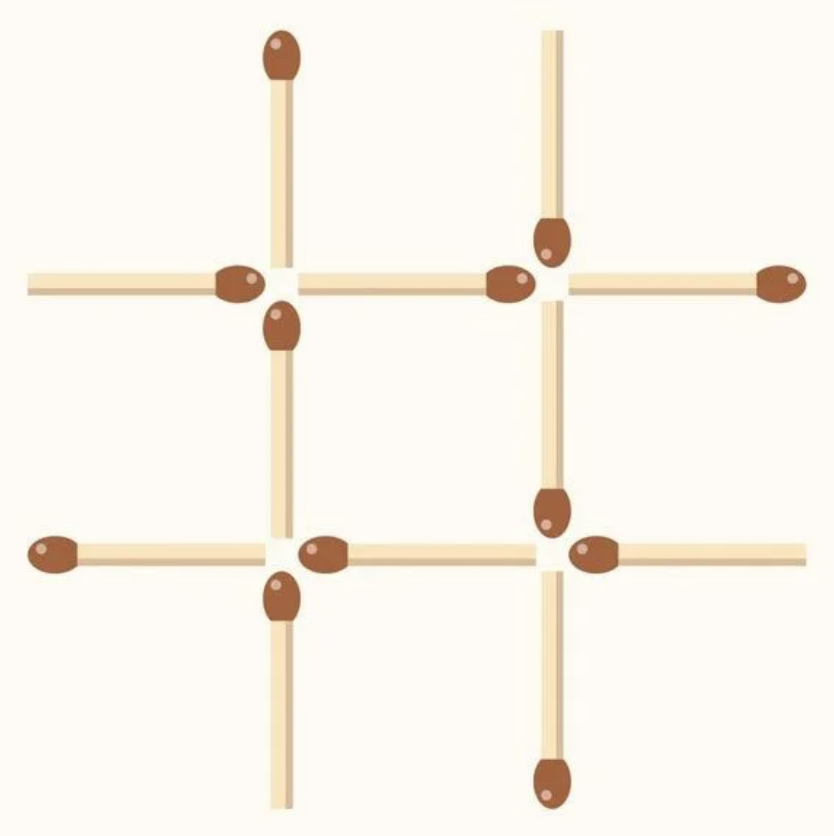
\includegraphics[width=0.3\linewidth]{spichki.png}
\end{figure}

\item 
a) Три пирата делят слитки золота весом $1,2,\dots,10$ килограммов. Могут ли они поделить золото поровну, если распиливать слитки запрещается? 

b) При дележе один из пиратов был убит. Могут ли два оставшихся пирата разделить золото поровну, если распиливать слитки по-прежнему запрещается?

\item Занятия кружка художественного свиста проходят по вторникам и четвергам. Оказалось, что в некотором месяце состоится 10 занятий этого кружка. На какой день недели приходится первое число этого месяца?

\end{enumerate}
\end{document}